\documentclass[10pt,twocolumn,letterpaper]{article}

\usepackage{iccv}
\usepackage{times}
\usepackage{epsfig}
\usepackage{graphicx}
\usepackage{amsmath}
\usepackage{amssymb}
\usepackage{subcaption}

% Include other packages here, before hyperref.

% If you comment hyperref and then uncomment it, you should delete
% egpaper.aux before re-running latex.  (Or just hit 'q' on the first latex
% run, let it finish, and you should be clear).
\usepackage[pagebackref=true,breaklinks=true,letterpaper=true,colorlinks,bookmarks=false]{hyperref}

 \iccvfinalcopy % *** Uncomment this line for the final submission

% Pages are numbered in submission mode, and unnumbered in camera-ready
\ificcvfinal\pagestyle{empty}\fi

\begin{document}

%%%%%%%%% TITLE
\title{CAP 5516 Medical Image Computing Spring 2022 Assignment 2: BraTS MRI Segmentation Challenge}

\author{Kyle Beggs\\
Department of Mechanical and Aerospace Engineering\\ 
University of Central Florida\\
{\tt\small kbeggs07@knights.ucf.edu}}

\maketitle
% Remove page % from the first page of camera-ready.
\ificcvfinal\thispagestyle{empty}\fi


%%%%%%%%%%%%%%%%%%%%%%%%%%%%%%%%%%%%%%%%%%%%%%%%%%%%%%%%%%%%%%%%%%%%%%%%%%%%%%%
\section{Problem Definition}

Segmentation of medical images is perhaps the most prevalent imaging task, so it is of great interest to continuously build motivation to push the boundaries of performance. Given a dataset of 3D MRI brain scans, we aim to segment the tumors present.


%%%%%%%%%%%%%%%%%%%%%%%%%%%%%%%%%%%%%%%%%%%%%%%%%%%%%%%%%%%%%%%%%%%%%%%%%%%%%%%
\section{Methods}
Since we are training on 3D images, and the assignment is to use a UNet type architecture, there are 2 main routes to go regarding architectures. You can use a 2D UNet and segment slice by slice or a true 3D UNet which uses 3D convolutions. We choose the latter because it is shown to perform better as you contain information in all dimensions for each operation which allows for better localization, although at the cost of extra computation. Here, we use the 3D UNet from \cite{kerfootLeftVentricleQuantificationUsing2019}.

\begin{figure}[h]
   \begin{center}
      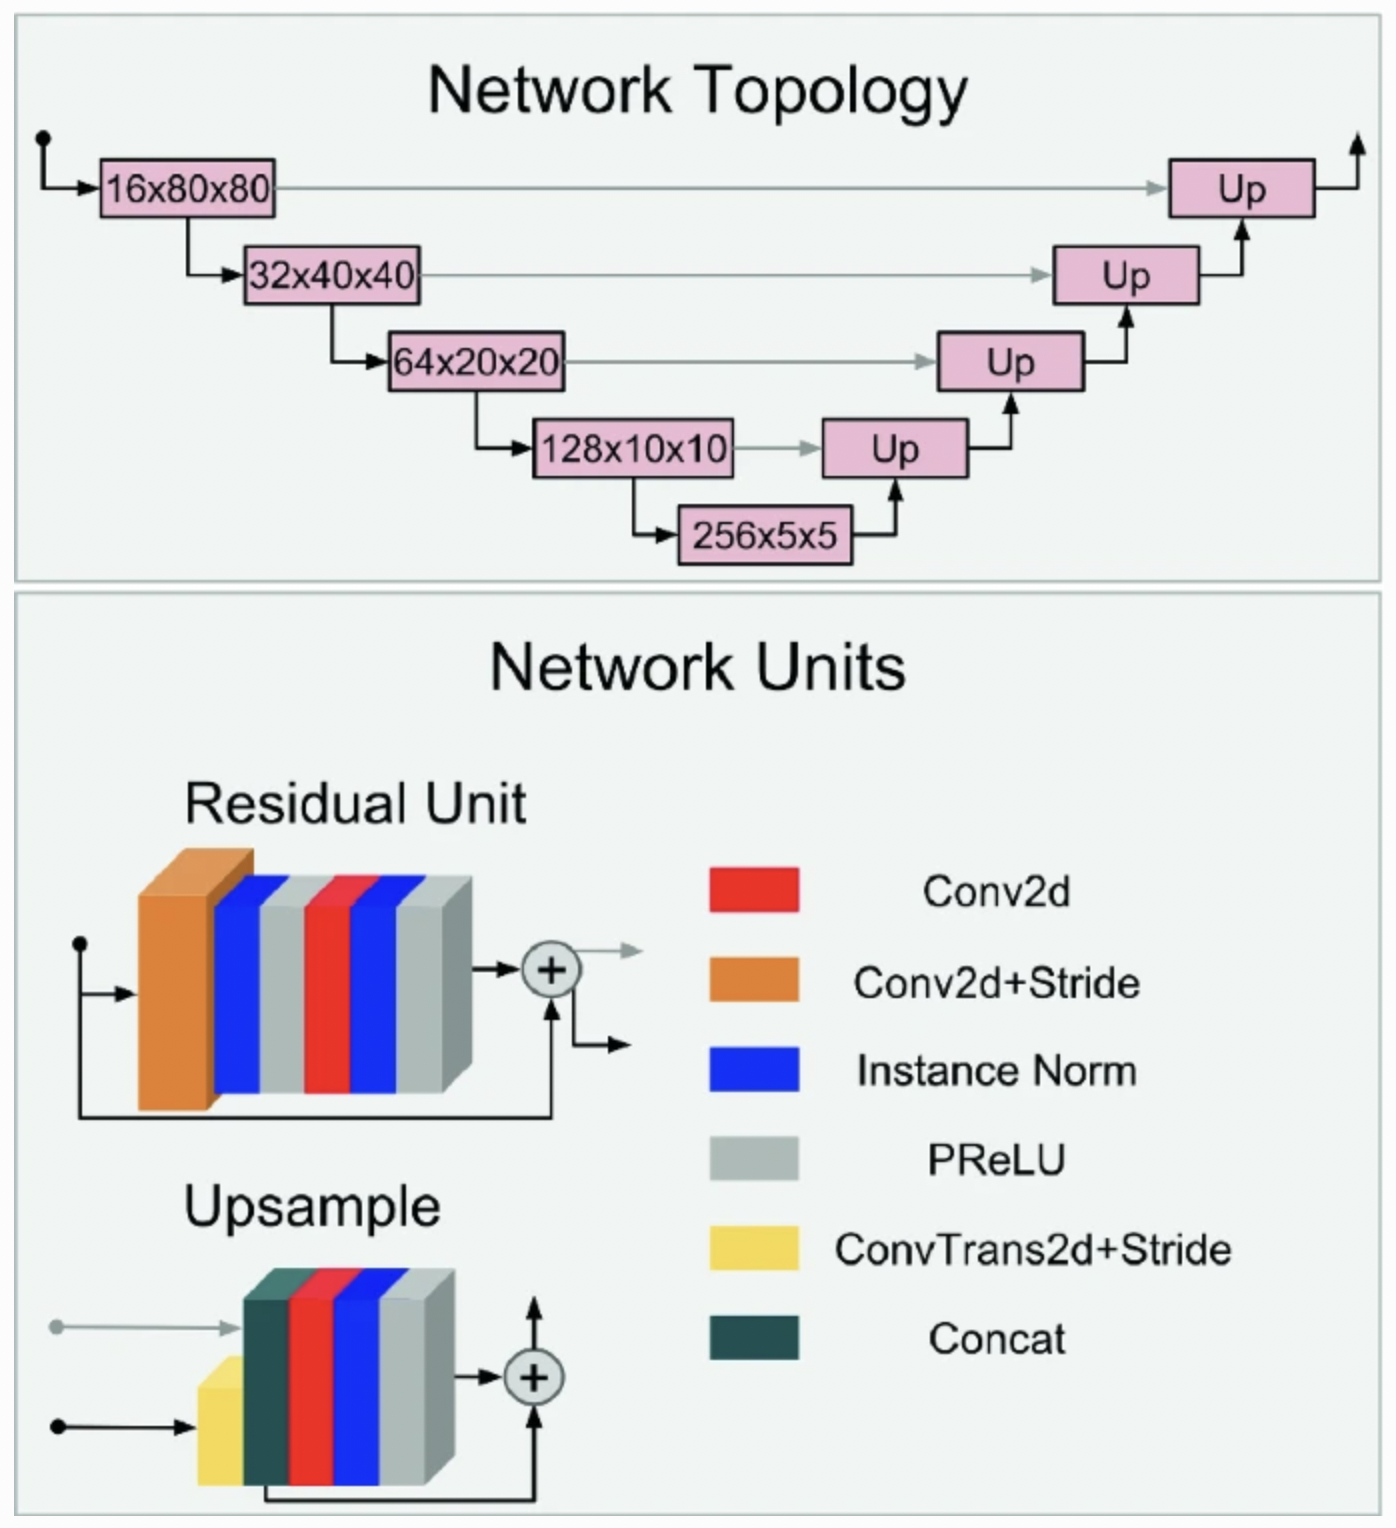
\includegraphics[width=0.95\linewidth]{images/network-arch.png}
   \end{center}
   \caption{3D UNet architecture with residual units.}
   \label{fig:arch}
\end{figure}

The dataset contains .nii.gz files which all the images are of the same size (240, 240, 155). Preprocessing of the data includes normalizing the intensity and augmenting by random flipping across all 3 axes, small random intensity shifts and scales, and a small random cropping of the image to a final size of (224, 224, 144).

The model was trained using 2 NVIDIA V100 16GB GPUs on the same node with a Cosine Annealing learning rate scheduler initialized at 0.001. The batch size was set to 8. K-Fold cross validation was used and the model was trained from random weight initialization for each fold. 5 folds were used. Some examples of the data are shown in figures \ref{fig: viz1} and \ref{fig: viz2}.

\begin{figure}[h]
   \begin{center}
      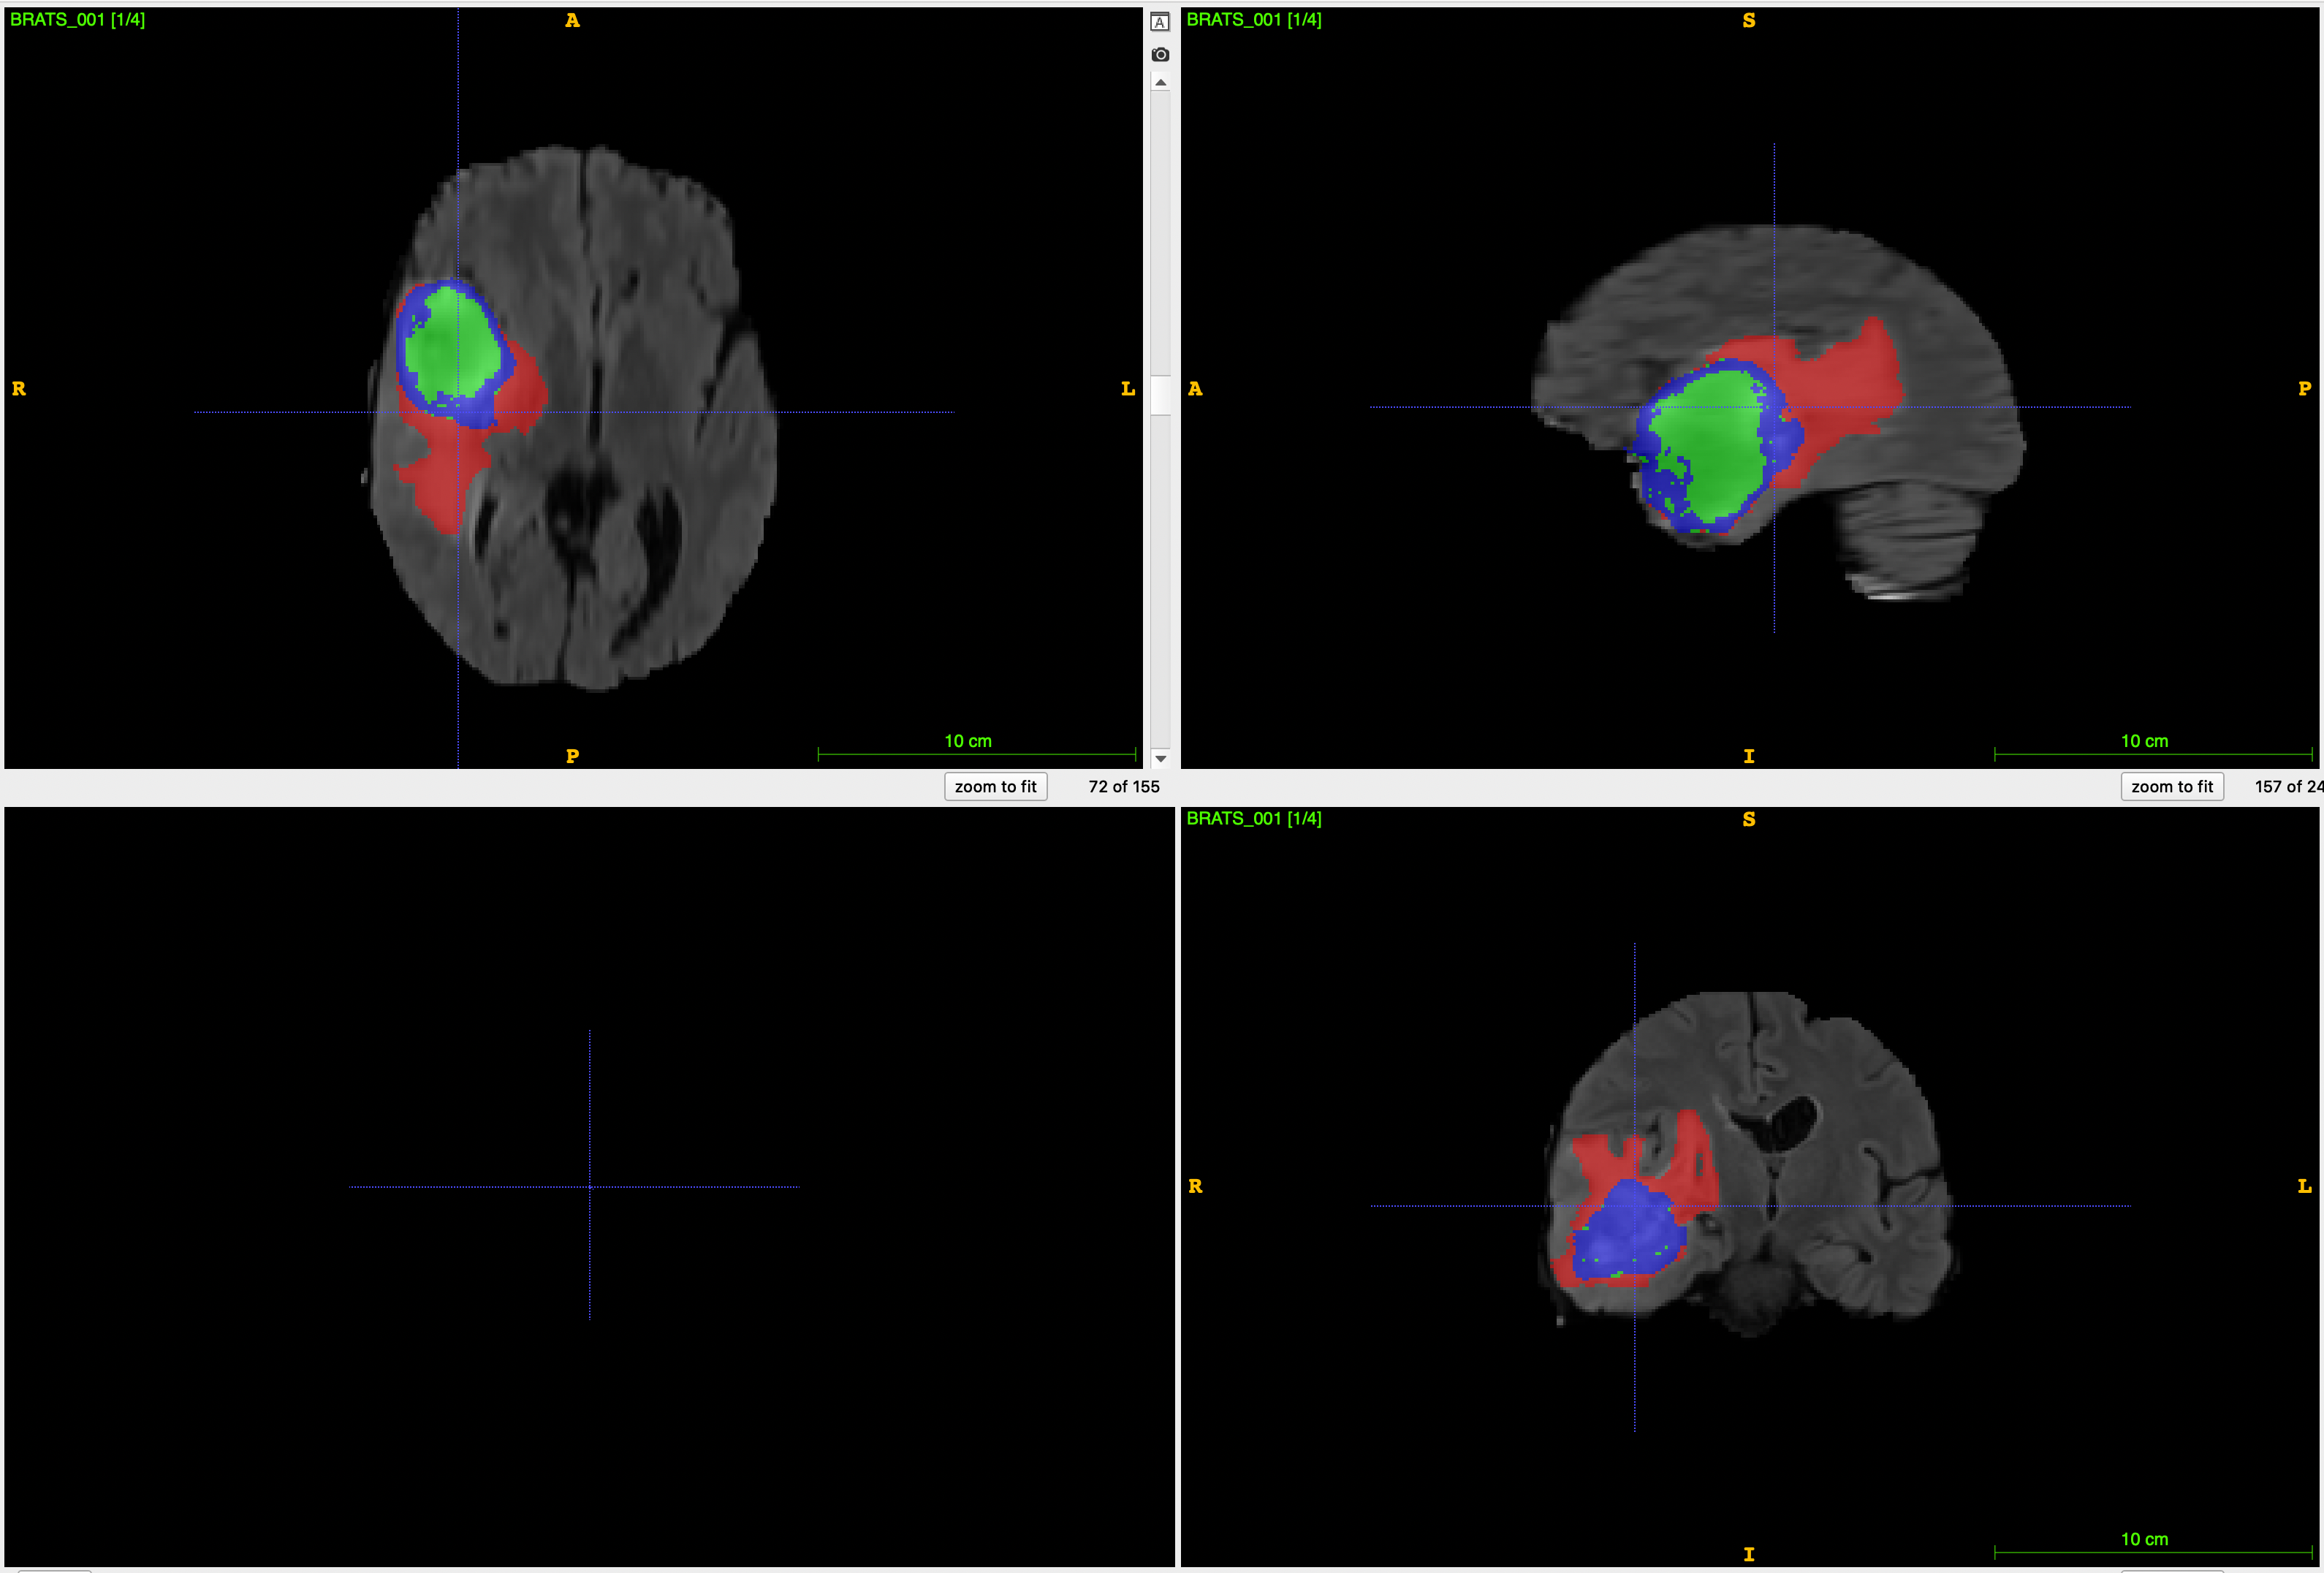
\includegraphics[width=0.95\linewidth]{images/visualization1.png}
   \end{center}
   \caption{Random visualization of the training image and label.}
\label{fig: viz1}
\end{figure}

\begin{figure}[h]
   \begin{center}
      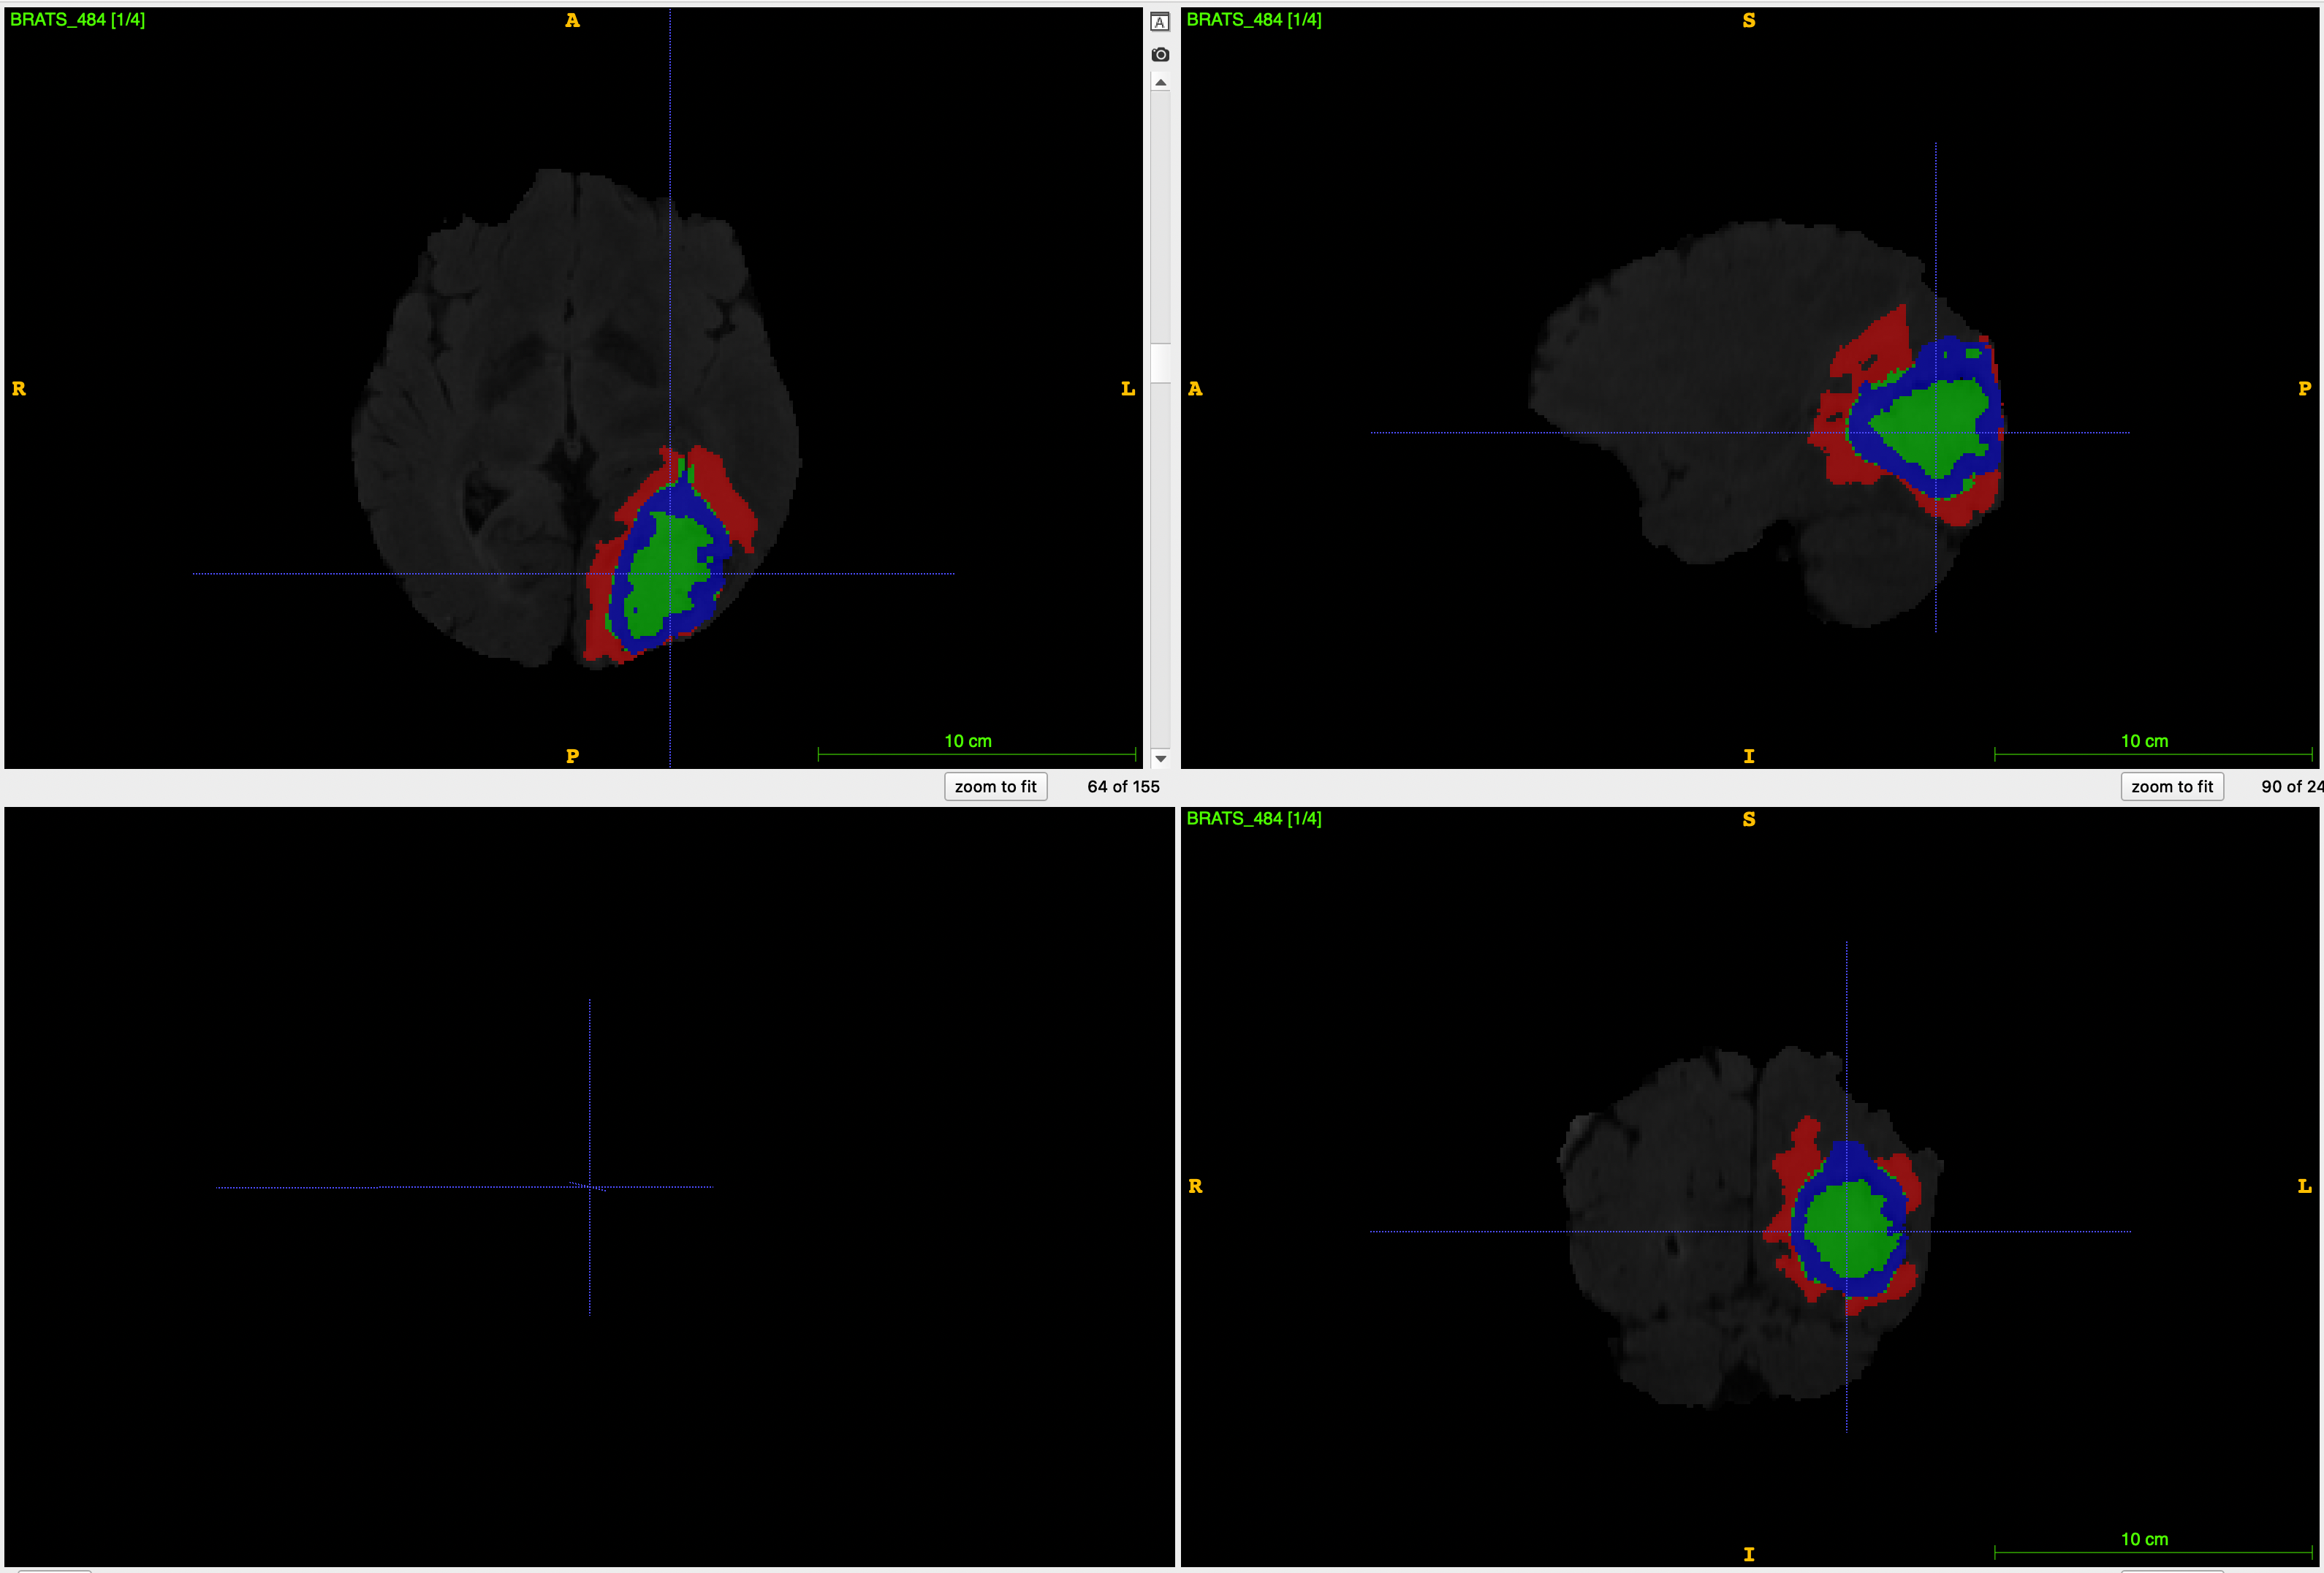
\includegraphics[width=0.95\linewidth]{images/visualization2.png}
   \end{center}
   \caption{Random visualization of the training image and label.}
\label{fig: viz2}
\end{figure}


%%%%%%%%%%%%%%%%%%%%%%%%%%%%%%%%%%%%%%%%%%%%%%%%%%%%%%%%%%%%%%%%%%%%%%%%%%%%%%%
\section{Results}

The validation set for each fold is evaluated and shown in Table \ref{table: dice and hausdorff}. The training loss for each fold is shown in figure \ref{fig: training loss}. Notice the pink line (fold 3) converges much slower than the other 4 folds, but does catch up by the end of the training. Interestingly enough, it ends up being the 2nd best performing fold.

\begin{table}[h]
   \begin{center}
       \begin{tabular}{l l l l l}
         Fold &
         \multicolumn{1}{p{2em}}{\centering Dice} &
         \multicolumn{1}{p{3em}}{\centering Hausdorff} \\
         \hline
         1 & 0.750 & 9.665 \\
         2 & 0.759 & 11.049 \\
         3 & 0.760 & 9.468 \\
         4 & 0.768 & 9.783 \\ 
         5 & 0.732 & 12.397 \\
         Avg. & 0.754 & 10.472
      \end{tabular}
   \end{center}
   \caption{Results of each cross fold. The Dice and Hausdorff values shown here are the averages of the 3 segmentations.}
   \label{table: dice and hausdorff}
\end{table}

\begin{figure}[h]
   \begin{center}
      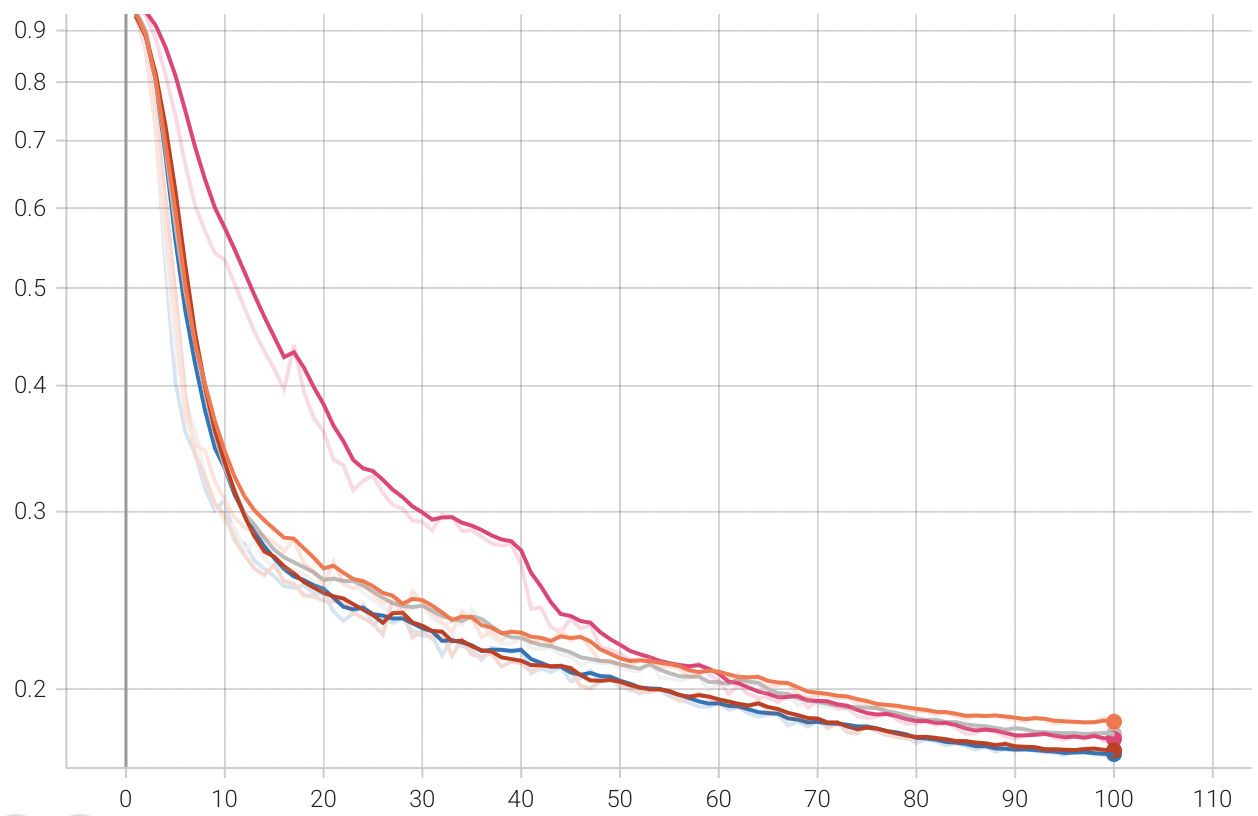
\includegraphics[width=0.95\linewidth]{images/training_loss.png}
   \end{center}
   \caption{Training loss curves for training set. fold (color): fold1 (orange), fold2 (red), fold3 (pink), fold4 (grey), fold5 (blue).}
\label{fig: training loss}
\end{figure}

Visualization of the models segmentation results using the weights found in fold 1 is seen in figures \ref{fig: viz result 1} and \ref{fig: viz result 2}.

\begin{figure}[!h]
	\begin{subfigure}{\textwidth}
		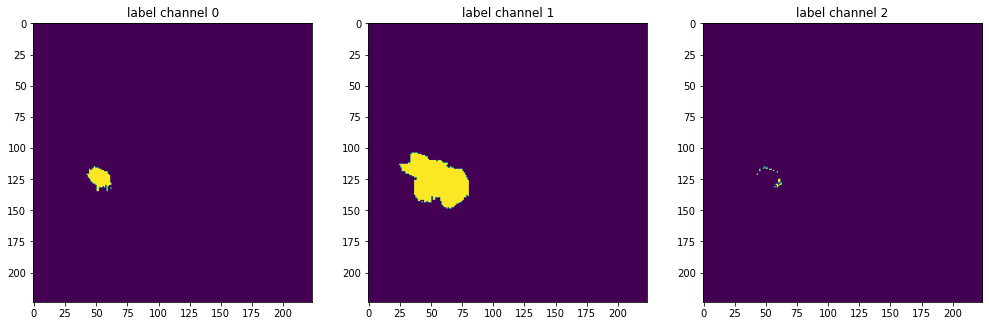
\includegraphics[width=0.5\linewidth]{images/outputvisualization1 - truth.png}
	\caption{Ground truth.}
	\end{subfigure}
	\bigskip
	\begin{subfigure}{\textwidth}
		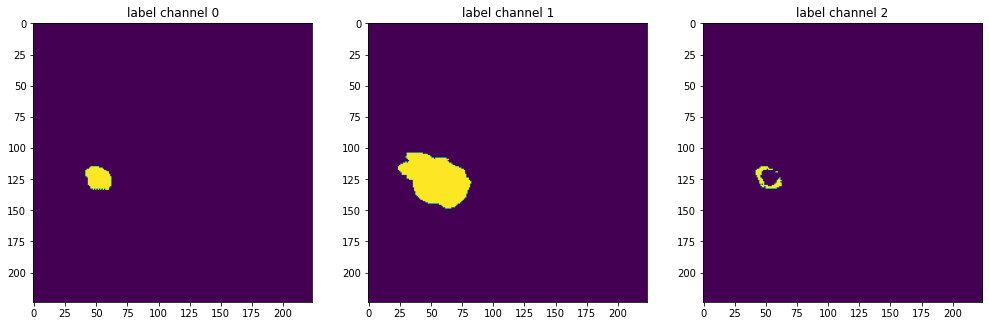
\includegraphics[width=0.5\linewidth]{images/outputvisualization1 - seg.png}
	\caption{Fold 1 segmentation.}
	\label{fig: viz result 1}
	\end{subfigure}
	\caption{Comparing ground truth to fold 1 segmentation.}
\end{figure}

\begin{figure}[!h]
	\begin{subfigure}{\textwidth}
		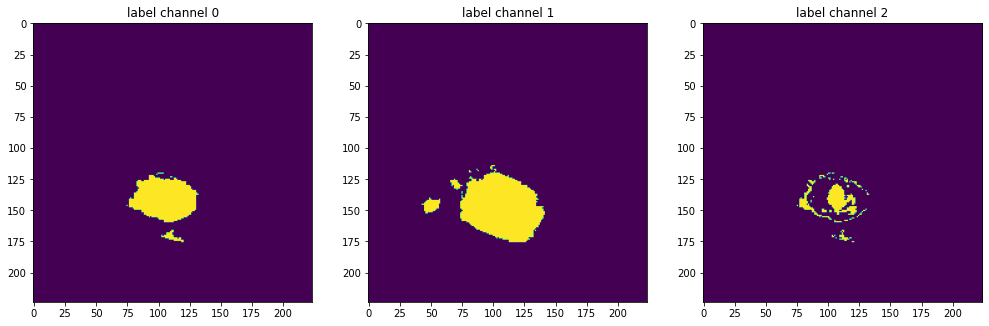
\includegraphics[width=0.5\linewidth]{images/outputvisualization2 - truth.png}
	\caption{Ground truth.}
	\end{subfigure}
	\bigskip
	\begin{subfigure}{\textwidth}
		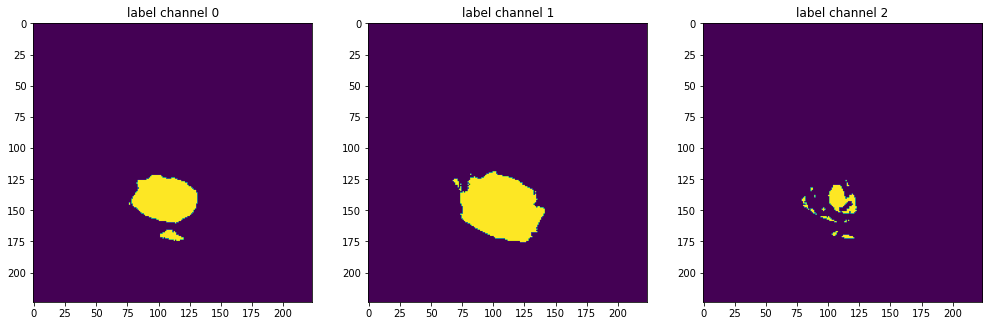
\includegraphics[width=0.5\linewidth]{images/outputvisualization2 - seg.png}
	\caption{Fold 1 segmentation.}
	\label{fig: viz result 2}
	\end{subfigure}
	\caption{Comparing ground truth to fold 1 segmentation.}
\end{figure}


%%%%%%%%%%%%%%%%%%%%%%%%%%%%%%%%%%%%%%%%%%%%%%%%%%%%%%%%%%%%%%%%%%%%%%%%%%%%%%%
\section{Discussion}

I have demonstrated the ability to successfully segment brain tumors using the BraTS dataset. K-fold cross validation is a good strategy to ensure you split the dataset into fair training/validation splits because some folds clearly performed better than others. Another big takeway is the large compute time; this training took ~22 hours for all 5 folds on 2 V100 GPUs only going to 100 epochs each fold. 

The code can be found on GitHub at \href{https://github.com/kylebeggs/Pediatric-Pneumonia-Classification-from-XRay}{kylebeggs/Pediatric-Pneumonia-Classification-from-XRay}.

{\small
\bibliography{UCF-course}
\bibliographystyle{IEEEtran}
}

\end{document}
